%%%%%%%%%%%%%%%%%%%%%%%%%%%%%%%%%%%%%%%%%%%%%%%%%%%%%%%%%%%
% EPFL report package, main thesis file
% Goal: provide formatting for theses and project reports
% Author: Mathias Payer <mathias.payer@epfl.ch>
%
% To avoid any implication, this template is released into the
% public domain / CC0, whatever is most convenient for the author
% using this template.
%
%%%%%%%%%%%%%%%%%%%%%%%%%%%%%%%%%%%%%%%%%%%%%%%%%%%%%%%%%%%
\documentclass[a4paper,11pt,oneside]{report}
% Options: MScThesis, BScThesis, MScProject, BScProject
\usepackage[MScProject]{EPFLreport}
\usepackage{xspace, xparse, amsmath, amssymb, dirtytalk}
\usepackage{svg}
\svgpath{{./img/}}
%\adviser{Prof. Dr. sc. ETH Mathias Payer} Maybe Vaudenay?
%\coadviser{Second Adviser}
%\expert{The External Reviewer}

\newcommand{\sysname}{M-SIDH\xspace}
\newcommand{\zp}{$\mathbb{Z}_p$\xspace}
\newcommand{\zn}{$\mathbb{Z}_n$\xspace}
\newcommand{\Fq}{$\mathbb{F}_q$\xspace}
\newcommand{\spc}{\hspace{0.5cm}}

\begin{document}
% Example of title page for the projects carried out within the lasec 

% Simply include it in your mastex tex file: 
%        % Example of title page for the projects carried out within the lasec 

% Simply include it in your mastex tex file: 
%        % Example of title page for the projects carried out within the lasec 

% Simply include it in your mastex tex file: 
%        \input{cover}


% Updated March 2006 (SP)


\newcommand{\logoepfl}[0]{
  \begin{center}
    
\includegraphics[width=4cm]{logo_epfl_coul.eps}
  \end{center}
  \vspace{0.3cm}
  \hrule
}
\newcommand{\logolasec}[0]{
  \vspace{1cm}
  \hrule
  \begin{center}
    
\includegraphics[width=4.5cm]{logo_lasec_coul.eps}
  \end{center}
}
\newcommand{\project}[1]{
  \begin{center}
    \large{#1}
  \end{center}
  \vspace{1cm}
}
\newcommand{\department}[1]{
  \begin{center}
    \large{#1}
  \end{center}
}
\newcommand{\supervisor}[3]{
  \begin{center}
    \begin{normalsize}{
        \bf #1}\\#2\\#3
    \end{normalsize}
  \end{center}
}
\renewcommand{\author}[1]{
  \begin{center}
    \Large{#1}
  \end{center}
  \vspace{0.5cm}
}
\renewcommand{\title}[1]{
  \vspace{3cm}
  \begin{center}
    \huge{#1}
  \end{center}
  \vspace{1.7cm}
}
\renewcommand{\date}[2]{
  \begin{center}
    \normalsize{#1 #2}
  \end{center}
  \vspace{0.5cm}
}


\thispagestyle{empty}


% begin title page
  \logoepfl
  
  \title{Implementing countermeasures for attacks on Supersingular Isogeny Diffie-Hellman (SIDH)}
  
  \author{Malo Ranzetti}
  \department{School of Computer and Communication Sciences}
  \project{Semester Project}
  
  \date{June}{2023}

  \begin{center}
    \begin{tabular}{cc}
      \begin{tabular}{p{4.0cm}}
        \supervisor{Responsible}{Prof. Serge Vaudenay}{EPFL / LASEC}
      \end{tabular}&
      \begin{tabular}{p{4.0cm}}
        \supervisor{Supervisor}{Dr. Boris Fouotsa}{EPFL / LASEC}
      \end{tabular}
    \end{tabular}
  \end{center}

\logolasec
% end title page




% Updated March 2006 (SP)


\newcommand{\logoepfl}[0]{
  \begin{center}
    
\includegraphics[width=4cm]{logo_epfl_coul.eps}
  \end{center}
  \vspace{0.3cm}
  \hrule
}
\newcommand{\logolasec}[0]{
  \vspace{1cm}
  \hrule
  \begin{center}
    
\includegraphics[width=4.5cm]{logo_lasec_coul.eps}
  \end{center}
}
\newcommand{\project}[1]{
  \begin{center}
    \large{#1}
  \end{center}
  \vspace{1cm}
}
\newcommand{\department}[1]{
  \begin{center}
    \large{#1}
  \end{center}
}
\newcommand{\supervisor}[3]{
  \begin{center}
    \begin{normalsize}{
        \bf #1}\\#2\\#3
    \end{normalsize}
  \end{center}
}
\renewcommand{\author}[1]{
  \begin{center}
    \Large{#1}
  \end{center}
  \vspace{0.5cm}
}
\renewcommand{\title}[1]{
  \vspace{3cm}
  \begin{center}
    \huge{#1}
  \end{center}
  \vspace{1.7cm}
}
\renewcommand{\date}[2]{
  \begin{center}
    \normalsize{#1 #2}
  \end{center}
  \vspace{0.5cm}
}


\thispagestyle{empty}


% begin title page
  \logoepfl
  
  \title{Implementing countermeasures for attacks on Supersingular Isogeny Diffie-Hellman (SIDH)}
  
  \author{Malo Ranzetti}
  \department{School of Computer and Communication Sciences}
  \project{Semester Project}
  
  \date{June}{2023}

  \begin{center}
    \begin{tabular}{cc}
      \begin{tabular}{p{4.0cm}}
        \supervisor{Responsible}{Prof. Serge Vaudenay}{EPFL / LASEC}
      \end{tabular}&
      \begin{tabular}{p{4.0cm}}
        \supervisor{Supervisor}{Dr. Boris Fouotsa}{EPFL / LASEC}
      \end{tabular}
    \end{tabular}
  \end{center}

\logolasec
% end title page




% Updated March 2006 (SP)


\newcommand{\logoepfl}[0]{
  \begin{center}
    
\includegraphics[width=4cm]{logo_epfl_coul.eps}
  \end{center}
  \vspace{0.3cm}
  \hrule
}
\newcommand{\logolasec}[0]{
  \vspace{1cm}
  \hrule
  \begin{center}
    
\includegraphics[width=4.5cm]{logo_lasec_coul.eps}
  \end{center}
}
\newcommand{\project}[1]{
  \begin{center}
    \large{#1}
  \end{center}
  \vspace{1cm}
}
\newcommand{\department}[1]{
  \begin{center}
    \large{#1}
  \end{center}
}
\newcommand{\supervisor}[3]{
  \begin{center}
    \begin{normalsize}{
        \bf #1}\\#2\\#3
    \end{normalsize}
  \end{center}
}
\renewcommand{\author}[1]{
  \begin{center}
    \Large{#1}
  \end{center}
  \vspace{0.5cm}
}
\renewcommand{\title}[1]{
  \vspace{3cm}
  \begin{center}
    \huge{#1}
  \end{center}
  \vspace{1.7cm}
}
\renewcommand{\date}[2]{
  \begin{center}
    \normalsize{#1 #2}
  \end{center}
  \vspace{0.5cm}
}


\thispagestyle{empty}


% begin title page
  \logoepfl
  
  \title{Implementing countermeasures for attacks on Supersingular Isogeny Diffie-Hellman (SIDH)}
  
  \author{Malo Ranzetti}
  \department{School of Computer and Communication Sciences}
  \project{Semester Project}
  
  \date{June}{2023}

  \begin{center}
    \begin{tabular}{cc}
      \begin{tabular}{p{4.0cm}}
        \supervisor{Responsible}{Prof. Serge Vaudenay}{EPFL / LASEC}
      \end{tabular}&
      \begin{tabular}{p{4.0cm}}
        \supervisor{Supervisor}{Dr. Boris Fouotsa}{EPFL / LASEC}
      \end{tabular}
    \end{tabular}
  \end{center}

\logolasec
% end title page



\begin{abstract}
Isogenies between supersingular elliptic curves are useful to construct cryptographic schemes that may be resilient in a post-quantum cryptographic era. One particular scheme proposed is the Supersingular Isogeny Diffie-Hellman (SIDH) key exchange. Since its proposal in 2011, it was seen as a promising candidate \cite{original-sidh}. However in 2022 it was shown that one can mount a devastating polynomial time attack against SIDH \cite{attack, robert}. Countermeasures to this attack have been proposed by Fuotsa, Moriya and Petit \cite{msidh}, but imply an explosion in the size of the scheme parameters. 

This project describes the implementation of one countermeasure, namely M-SIDH, for which we implement parameter generation and key exchange for an arbitrary security parameter $\lambda$. After evaluating the system performance, we come to the conclusion that for most practical purposes, these new proposed schemes demand an extreme amount of computational power relative to the security they provide. Making them a viable cryptosystem would require a more efficient algorithm to compute isogenies of large separable degrees. Parameter generation is also affected as we would likely need a third party to pre-compute parameters long in advance.
\\ \\
\textbf{Keywords:} M-SIDH, SIDH, Post-Quantum Cryptography, Elliptic Curves
\\ \\
\textbf{Maintained repository:} \href{https://github.com/mrztti/lasec-MSIDH}{github.com/mrztti/lasec-MSIDH}
\end{abstract}

\maketoc

%%%%%%%%%%%%%%%%%%%%%%
\chapter{Introduction}
%%%%%%%%%%%%%%%%%%%%%%

In recent years, the study of isogenies between supersingular elliptic curves has gained significant attention in the field of post-quantum cryptography. Isogenies provide a powerful mathematical tool for constructing cryptographic schemes that are believed to be resistant against attacks by quantum computers. One of the previously most promising schemes in this area was the Supersingular Isogeny Diffie-Hellman (SIDH) key exchange, which was first proposed in 2011 \cite{original-sidh}.

The SIDH key exchange relies on the properties of supersingular elliptic curves and isogenies to establish a shared secret between two parties over a public channel. However, in 2022, a devastating polynomial time attack against SIDH was discovered \cite{attack, robert}. As a result, countermeasures have been proposed to mitigate this attack, such as the M-SIDH scheme, introduced by Fuotsa, Moriya, and Petit \cite{msidh}.

This project focuses on the implementation of M-SIDH and its evaluation in terms of performance. M-SIDH addresses the vulnerability exploited by the attack on SIDH by modifying the computation of the public keys to prevent the attacker from obtaining crucial information. The implementation includes the parameter generation and key exchange for an arbitrary security parameter $\lambda$. The system's performance is evaluated to assess its practicality for real-world applications.

During the implementation and evaluation process, it becomes apparent that the computational requirements of M-SIDH are prohibitively high for most practical purposes. The schemes proposed by Fuotsa, Moriya, and Petit demand a significant amount of computational power relative to the level of security they provide. Additional progress in developing efficient algorithms for computing isogenies with large separable degrees is necessary to enhance the viability of these cryptosystems. Moreover, the generation of parameters would probably entail pre-computation conducted by a trusted third party well ahead of time (probably as a service, so that the parameter computation burden is removed from the exchanging parties). This is also for reasons mentioned in \autoref{endo_remark}, specifically that it may be needed for the starting curve of the scheme to be constructed by a trusted third party.

In this paper, we present the design and implementation details of M-SIDH, along with the modifications made to the original scheme. We discuss the efficiency challenges faced during the implementation as well as the optimizations made to the mathematical programming framework. The limitations and implications of M-SIDH are also discussed, highlighting why there is a need for more efficient algorithms and more design work on the parameter generation process.

%%%%%%%%%%%%%%%%%%%%
\chapter{Background}
%%%%%%%%%%%%%%%%%%%%

A detailed and thorough mathematical background can be found in the original M-SIDH proposal paper \cite{msidh}. Here, we give an intuitive description of the main mathematical tools relating to the project, in the hope of making this project more available without full understanding of some high-level mathematical concepts.

\section{Diffie-Hellman Key Exchange}

    The Diffie-Hellman (DH) key exchange is a well documented and widely used mathematical construction which allows two parties to agree on a cryptographic key across a public channel. The scheme relies on the ability of the participating parties to construct secret, commutative trapdoor functions. \autoref{fig:dh_example} illustrates the idea behind the scheme \cite{dhmedia}.

    \begin{figure}[htp!]
        \centering
        \includesvg[inkscapelatex=false, width=150pt]{DH}
        \caption{Illustration of the concept behind the DH key exchange \cite{dhmedia}}
        \label{fig:dh_example}
    \end{figure}

    While the most popular implementation of this scheme is based upon modular exponentiation in the group \zp with a large prime $p$ as the secret trapdoor functions, SIDH uses an elliptic curve as a starting element and elliptic curve isogenies as the one-way functions. 

\section{Elliptic curves, Supersingularity \& Isogenies}

    Elliptic curves are characterized by their equation, given in the form (Weierstrass equation):

    \begin{equation}
        y^2 + a_1 x y + a_3 y = x^3 + a_2 x^2 + a_4 x + a_6
    \end{equation}

    When we take the given equation over a commutative ring, such as a finite field \Fq, we obtain a set of points that constitutes an Abelian group. In the general case, this group is not guaranteed to have the same order as the original commutative ring and furthermore it may be hard to calculate (although we can find lower and upper bounds using Hasse's theorem). This is one of the reasons why supersingular elliptic curves are handy: for a prime $p$, a supersingular curve $E$ over the finite field \Fq defines an Abelian group of points of order $p+1$. We can also further extend this to the case where we take the finite field $\mathbb{F}_{p^2}$: now we have an Abelian group isomorphic to $\mathbb{Z}_{p+1} \times \mathbb{Z}_{p+1}$ \cite{algorithms} for which we can find a basis $\left \langle P,\: Q \right \rangle$ with both points having order $p+1$.

    An isogeny is essentially a morphism ("map") between two curves (or possibly to itself). Isogenies are determined (up to isomorphism) by their kernel. The degree of an isogeny can be seen as the cardinality of its kernel. One interesting point is that the higher the isogeny degree, the more computationally complex it becomes to compute. We can also separate isogenies of composite order into a chain of isogenies of prime order in the factors of the original isogeny (which we use to calculate large isogenies efficiently).

    Isogenies between elliptic curves are not a commutative operations "as-is", but if we know the image of basis points of the isogeny kernel, we can fix the image curve such that the operation becomes "commutative" for our needed cryptographic purposes.

    
\section{Supersingular Isogeny Diffie-Hellman}

    As previously mentioned, SIDH replaces computations in the \zp  group with arithmetic over elliptic curves defined over a finite field $\mathbb{F}_q$ where $q=p^2$. 

    The \textbf{public parameters} include the curve, the integer $p$ and importantly the values used to generate it $A,B$ which correspond to the degrees of the isogenies used by the two parties. The torsion points of the $A,B$-torsion subgroup of the curve over the finite field are also made public. Concretely, this means that both parties disclose a basis for the respective starting kernel of their secret isogeny.
    Now, the public keys consist of the image of the base curve $E_0$ given by a secret isogeny of high degree, for each party. Along with the curve, each party must transmit the image of the other party's torsion points through their secret isogeny.
    Using these point images, the parties can apply their isogeny (albeit on a different pre-image domain) a second time on the received public key to each obtain a final curve. The shared secret, the j-invariant of the resulting curves, is then the same for both parties and can be used as a shared secret key.

    \textbf{Full specification:} For the complete and exact details of the protocol, see the original SIDH paper \cite{original-sidh}.

\section{Overview of the attack on SIDH}
\label{attack}

    In 2022, Castryck and Decru proposed a devastating attack on SIDH \cite{attack}. Additional work by Maino, Martindale and Robert led to a polynomial attack for an arbitrary starting curve $E_0$ \cite{robert}. The attack leverages the following key point: there exists an efficient oracle, that for a given step in the factored isogeny construction from the starting curve, decides if it is the correct step taken in the secret isogeny. In SIDH the secret isogenies can be separated into steps of 2- or 3-isogenies. Note that for an isogeny of degree n, there are n possible corresponding possible curves to be checked (if one omits the dual isogenies for each step).
    
    This oracle is constructed using a complex theorem (Kani's theorem) \cite{attack}. However it requires two main conditions to work \cite{msidh}:
    \begin{itemize}
        \item The degree $A$ of the secret supersingular isogeny $\phi : E_0\rightarrow E$ must be known.
        \item The images $\phi (P), \phi (Q)$ of the torsion basis $\left \langle P,\: Q \right \rangle$ of the B-torsion $E_0 [B]$ (where $B > A$ and are coprime) must be known.
    \end{itemize}
    
    As a consequence, countermeasures target either one of these conditions.

\section{Proposed countermeasures}

    Two countermeasures have been proposed in response to the attack on SIDH \cite{msidh}: M-SIDH (masked torsion points) and MD-SIDH (masked degree). However, we only focus on the M-SIDH variant, as for the same level of security, it makes use of isogenies of much lower degree\footnote{The prime $p$ used in MD-SIDH for NIST security level 1 is around as large as the prime used for M-SIDH security level 5 (around 13,000 bits) \cite{msidh}. As we see in \autoref{results:ke}, key exchange for this large prime is unreasonable for most modern applications.}. 

    M-SIDH proposes a defense against the attack (\autoref{attack}) by removing one of the necessary ingredients for its success: the images of the torsion points. Indeed, the SIDH protocol is modified by ensuring that the direct images of the torsion points are not available to the attacker, but that the curves resulting from the executed protocol still have the same j-invariant.

    Two main modifications are done in order to achieve this. The first one is that we scale the images of the torsion points by an integer $\alpha$ sampled randomly as follows:

    \begin{equation}
        \alpha \in_{R} \mu _ 2 (N):= \left \{  x \in \mathbb{Z}/N\mathbb{Z} \textup{ st. } x^2 \equiv 1 \left ( \textrm{mod } N\right )   \right \}
    \end{equation}

    The correctness of this scheme is proven in \cite{msidh-original} and comes down to the fact that the scaled torsion points generate the same kernel as the direct images. However, if the attacker can find the scaling factor $\alpha$, then they can run the attack. 

    There is an existing strategy to recover $\alpha ^2$ modulo the isogeny degree \cite{msidh-original}. Therefore, the security of M-SIDH relies on the fact that the multiplicity of the square roots of $\alpha$ modulo either isogeny degrees grows exponentially according to a security parameter $\lambda$. Therefore we must construct each isogeny degree as a product of distinct primes linearly in the parameter $\lambda$ (because the amount of square roots depends on the amount of prime factors of the modulus), so that exhaustive search of $\alpha$ becomes hard. Unfortunately, this means that the size of $p$ grows faster than factorial in $\lambda$ (indeed, the product of the first n primes is greater or equal to the product of the first n consecutive integers). This has consequences in terms of computation efficiency of the protocol, as we will see in this project.



%%%%%%%%%%%%%%%%%%%%%%%%
\chapter{Design and Implementation}
%%%%%%%%%%%%%%%%%%%%%%%%

The main goal of this project is to provide a proof of concept regarding practical use of M-SIDH. It is not a fully efficient and optimized implementation of M-SIDH, but does allow us to evaluate the practical cost on usability of applying a countermeasure on the original SIDH protocol. Although the most was done in the given time frame to implement as many efficiency optimizations as possible, there seems to be space to push the protocol some more to faster speeds as discussed in \autoref{discussion:limitations}.

\section{Use of SageMath Library}

    As a proof of concept, the project uses SageMath \cite{sagemath} for better readability and modularity. This framework will allow us to benefit from many already implemented computation strategies and provides decent computational efficiency. For example, SageMath implements an algorithm to compute isogenies of high, smooth degree, which is key to implement SIDH efficiently.
    
\section{Implementation of SIDH}

    We provide an implementation of SIDH using the same primitives and abstractions as our implementation of M-SIDH. This was done in order to have a fair comparison of the efficiency difference between the two strategies. The implementation comes equipped with a generalized interface abstraction to simulate Diffie-Hellman key exchange schemes.
        
\section{Implementing M-SIDH}

    \subsection{Modifications compared to proposed scheme}

    Some modifications were made or attempted during the implementation compared to the scheme as strictly proposed in \cite{msidh}. For example, the high level description of the public parameter selection algorithm as given in the original paper does not yield the expected primes described. The fault was identified as a wrong condition with respect to the security parameter $\lambda$. Indeed, it seems that instead of \textit{\say{ If $\lambda < t - n + 1$, we restart with a larger $t$} }[pg. 21], the correct condition should be $\lambda > t - n + 1$. While a direct proof is not included here, the implementation provides a script that illustrates this statement in practice (\texttt{t\_selection\_proof.sage}).

    Another modification which was made was to omit the $2^2$ factor present in the public parameter $A$ as given in the original paper \cite{msidh}. Note that this change was also made in another implementation \cite{compression}. This was done to enable use of the \texttt{velusqrt} algorithm \cite{velusqrt}, as to use this algorithm a requirement is that $A$ and $B$ must be of separable and odd degree. After many attempts, it seems that something isn't right in the Sage \texttt{velusqrt} implementation as discussed in \autoref{discussion:limitations}, and so this change was dropped.

    A final addition for parameter generation was to include a check relative to the base curve used. Indeed, if we take the example of the elliptic curve with j-invariant $1728$, we need that $p \equiv 3 \textrm{ mod } 4$ as an additional condition if we want our curve to be supersingular. We therefore add this check in the cofactor $f$ generation step. Note that similar varying conditions might be necessary depending on the choice of the base curve, and that the $2^2$ factor present in the public parameter $A$ is usually there to guarantee this specific condition.

    \textbf{Important remark:}
    \label{endo_remark}
    As noted in \cite{msidh}, the security of M-SIDH relies in part on the fact that the endomorphism of the starting curve $E_0$ should be unknown to an attacker. To achieve this, the cited paper proposes the possibility that a trusted third party could generate a random trusted supersingular starting curve using a random walk in the graph of supersingular isogenies. For simplicity's sake, we do not include this important point in the parameter generation implementation, but we do mention some implications in the concluding remarks.

    \subsection{Implementation efficiency hurdles}

    From early on in the project, it became clear that the biggest efficiency hurdles towards lower computation times in the implementation of M-SIDH were the calculations of generators of the base curve, sampling roots of unity of \zn and the isogeny computations of the two parties. An enormous amount of tweaking and perfecting was made to finally be able to arrive at decent computation times. The first naive implementation of M-SIDH at the beginning of the project used to have computation times in the order of 5 minutes for both parameter generation and key exchange with $\lambda = 32$. The current implementation is now around $10$ times faster for the same security parameter.

\section{Improving the Efficiency of M-SIDH}

    \subsection{Improving parameter generation}

    Whereas SIDH parameters are considered to be entirely public and reusable, it is interesting to focus on the efficiency of parameter generation of M-SIDH (and MD-SIDH as well) since a functional implementation could potentially require the use of arbitrary curves with non-public endomorphism rings \cite{msidh}. The bottleneck computation of parameter generation comes from the computation of basis points of the torsion subgroups of the chosen curve. The strategy we employ is based on the SIDH paper \cite{original-sidh} and \cite[Corollary 24.31]{pairing}: we randomly sample a point on the curve until we find one of order $p+1 = A\cdot B \cdot f$, which we denote P. We do the same for a distinct point Q. We use the properties of Weil pairings to check the linear dependence between the two points, and adjust our point Q until we have two linearly independent points that form a basis of $E(F_{ p^{2}})$. We finally multiply these points by $\frac{p+1}{A}, \frac{p+1}{B}$ respectively to obtain the desired torsion points.

        \subsubsection{Checking the order of a point}
    
        Because the base curve is supersingular, we know that $E(F_{ p^{2}}) \cong \mathbb{Z}_{p+1} \times \mathbb{Z}_{p+1}$. Instead of computing the exact order of a point, it is sufficient to check that the order of a possible point is exactly $p+1 = A \cdot B \cdot f$. To do this, we construct the following vector:
    
         \begin{displaymath}
         \label{eq:lp_star}
             LP^* = \begin{bmatrix}\frac{p+1}{l_i} \cdot P \textrm{  for } l_i \textrm{ the prime factors of } p+1\end{bmatrix} 
         \end{displaymath}
    
        If none of the elements of the vector are the point at infinity, then P is of order $p+1$. Indeed, we can argue from the previously mentioned isomorphism that the maximal order of any point in the curve group has a maximum order of $p+1$ and must also divide this value. Therefore, we can rule out all possible order values by checking if P multiplied by any of the largest divisors of $p+1$ (ie. all the $\frac{p+1}{l_i}$) results in the point at infinity. 

        This technique also allows us to pre-compute values that we reuse to construct the following vector used in later steps:

        \begin{displaymath}
         \label{eq:lp}
             LP = \begin{bmatrix}\frac{p'}{{l_i}^{e_i}} \cdot P \textrm{  for } {l_i}^{e_i} \textrm{ the prime factors of } p'\end{bmatrix} 
         \end{displaymath}

         Indeed, we can obtain $LP^*$ by further multiplying elements with non-zero prime factor exponents (there are typically very few of them) by the corresponding remaining factor. We use the same techniques to generate a point Q.


        \subsubsection{Checking linear independence}

        To check the linear independence of two points P, Q we use the previously constructed vectors $LP,\: LQ$ derived from \autoref{eq:lp}. We then compute the Weil pairing between each pair of values from theses vectors. If the two points are linearly independent, the paring value must have a multiplicative order of $l_i^{e_i}$. If we do encounter a pair of values for which the this test fails, then we know that we must adjust our candidate Q. Adjusting the point Q is faster than generating a new random point Q, checking that the order is $p+1$ and generating $LQ$ once more. 
        The adjustment is made the following way: let $LP_i$ correspond to the failed pairing value:

        \begin{enumerate}
            \item Sample a new random point R on the curve, then multiply it by $\frac{p+1}{{l_i}^{e_i}}$.
            \item Compute the Weil pairing of R and $LP_i$, and restart if it still is the pairing check still fails.
            \item Set $Q=Q-R$
        \end{enumerate}

        After doing this for every failed value, we can recompute the $LQ$ and check for peace of mind that our adjusted point Q is now linearly independent from P. This algorithm is a better choice since the calculation of the vectors $LP, LQ$ become the biggest bottlenecks when generating basis points for very large $p$. If we were to sample a new Q every time the check fails, we would have to calculate $LQ$ a large number of times before we would eventually fall on a valid point with enough luck. This algorithm is also much faster than a naive call to the SageMath \texttt{gens()} function as we leverage the specific construction of the group.
        

    \subsection{Sampling of square roots of unity in \zn}

    The naive implementation of sampling a random element of \zn and checking if it is indeed a square root of unity is highly inefficient. In the implementation given in \cite{msidh}, the only values of n for which we need to implement this sampling function are $n=A,B$. Because we have the factoring of these two values available to us, we can implement $\mu_2$ efficiently (function \texttt{mewtwo} in codebase). 
    We create an empty list to store values. We proceed by sampling a random bit $b$ uniformly for each factor $k$ of $n$ (available to us. Then, if $b=0$ we add $1$ to our list, otherwise if $b=1$ we add $k-1$. Finally we use the CRT between the items in our list in their corresponding factors as moduli to deduce our final result.

    \subsection{Implementation usage guide}

    The implementation provides a main entry point \texttt{run.py} which must be run using a recent version of Sage \cite{sagemath} and given arguments. Note that to obtain the performance as evaluated in this report, one must modify the Sage source code for factored isogeny computation as described in \autoref{discussion:limitations}. The outputs of all tests are saved to a CSV file.

    \textbf{Example use cases}
    \begin{itemize}
    
        \item Show help: \\ \texttt{sage run.py -h}
        \item Run SIDH implementation on p751 parameters: \\ \texttt{sage run.py -t sidh -c p751}
        \item Generate M-SIDH parameters for $\lambda = 128$ as given in \cite{msidh}: \\ \texttt{sage run.py -g128}
        \item Generate M-SIDH parameters for arbitrary $\lambda$ given as an argument \cite{msidh}\\ \texttt{sage run.py -g <lambda>}
        \item Test 2 rounds of M-SIDH using the parameters for $\lambda = 128$: \\ 
        \texttt{sage run.py -t msidh -r 2 -f MSIDHp128.pickle}
        \item Test 10 rounds of M-SIDH using the parameters for arbitrary $\lambda = 32$: \\ 
        \texttt{sage run.py -t msidh -r 10 -f MSIDH\_AES-32.pickle }
        
        
    \end{itemize}



%%%%%%%%%%%%%%%%%%%%
\chapter{Evaluation}
%%%%%%%%%%%%%%%%%%%%

The evaluation of this implementation consists of a time based analysis. In most modern cryptosystems, it can be argued that the most decisive factor to determine usefulness is computation time proportional to security level. We will evaluate both the generation of parameters and the key exchange. 

\textbf{System specifications:} The evaluation was performed on a M2 pro Apple silicon (12 cores 3.3GHz, 16GB RAM)


\section{Parameter Generation}

    As we can see in \autoref{result:gen_table}, the results for parameter generation are already quite alarming. Indeed, parameter generation for classical NIST-1 level security already takes around 2000 seconds. As we see in \autoref{fig:gen1}, the parameter generation time is exponential relative to the security parameter. Fitting an exponential curve to the results obtained (\autoref{fig:gen2}) we can estimate that generating parameters for $\lambda = 192,\:256$ should take more than 5 hours and more than a day respectively. For time's sake, we will therefore omit the evaluation for these values (especially since the next section shows that cost of performing the key exchange grows even faster than parameter generation).
    
    \begin{table}[!h]
        \label{result:gen_table}
        \begin{center}
        \begin{tabular}{| c | c |}
        \hline
        \textbf{$\lambda$ (bits)} & \textbf{Generation time (s)}  \\ 
        \hline

        4 & 0.09961 \\ \hline
        8 & 0.5185 \\ \hline
        16 & 1.901 \\ \hline
        32 & 25.55 \\ \hline
        64 & 303.6 \\ \hline
        128 & 2026 \\ \hline
        \hline
        \end{tabular}
        \end{center}
        \caption{Evaluation of parameter generation (5 repetitions)}
    \end{table}

    \begin{figure}
        \centering
        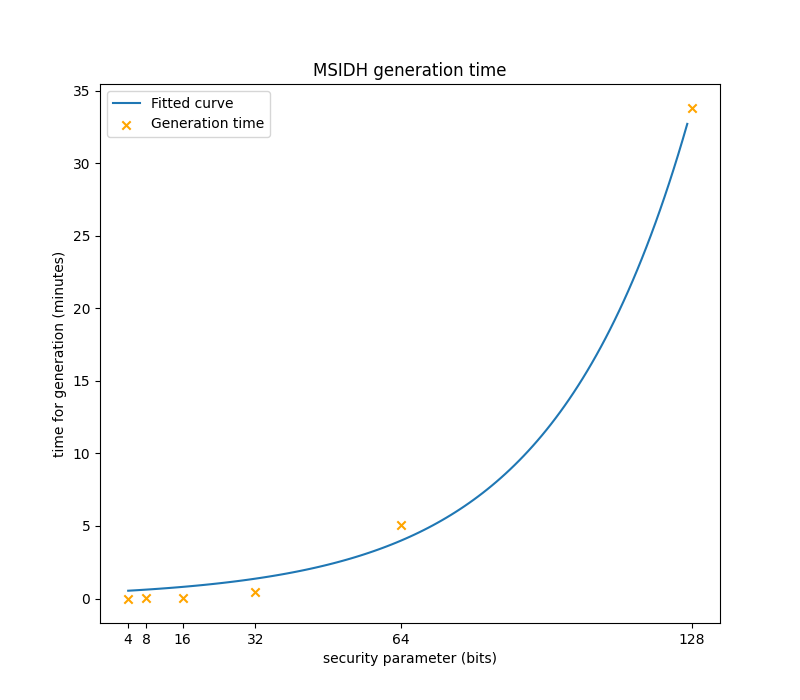
\includegraphics[width=0.7\textwidth]{img/Figure_3.png}
        \caption{Plot of parameter generation times}
        \label{fig:gen1}
    \end{figure}

    \begin{figure}
        \centering
        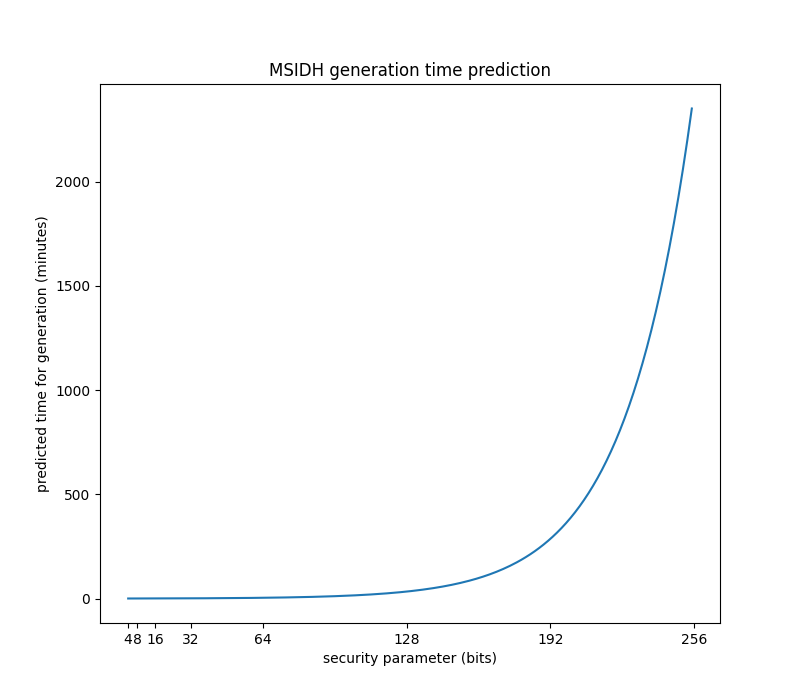
\includegraphics[width=0.7\textwidth]{img/Figure_4.png}
        \caption{Prediction of generation times}
        \label{fig:gen2}
    \end{figure}
    

\section{Key exchange}
\label{results:ke}

    \begin{table}[!h]
        \label{result:ex_table}
        \begin{center}
        \begin{tabular}{| c | c |}
        \hline
        \textbf{$\lambda$ (bits)} & \textbf{Key exchange time (s)}  \\ 
        \hline

        4 & 0.1681 ± 0.0028\\ \hline
        8 & 0.8171 ± 0.013\\ \hline
        16 & 4.183 ± 0.070\\ \hline
        32 & 28.27 ± 0.47\\ \hline
        64 & 252.5 ± 4.2\\ \hline
        128 & 3000 ± 50\\ \hline
        \hline
        \end{tabular}
        \end{center}
        \caption{Evaluation of parameter generation (20 repetitions)}
    \end{table}

    After evaluation, we obtain similar results for the full key exchange protocol in the sense that the time needed to complete the protocol grows exponentially as the security parameter (and thus $p$) grows. Even using the smallest parameter proposed in \cite{msidh} yields computation times that are way beyond most practical uses of the cryptosystem (for this implementation at least). The total sum of the computation time, as shown in \autoref{result:ex_table}, is of around 3000 seconds (50 minutes). 
    
    
    
    These results are not so far from the results obtained in \cite{compression}. As a point of reference, completing one full exchange using SIDH as implemented in this project takes around 10 seconds for NIST security level 5 (curve \texttt{p751}). If we consider that both parties can compute the isogenies simultaneously, we can consider that this means a practical exchange could happen in 25 minutes. From the results, plotted in \autoref{fig:ex1}, we can see that the key exchange is even more computationally expensive than the parameter generation. We show an estimate\footnote{Estimated by fitting an exponential curve to points sampled up to $\lambda = 128$ bits} in \autoref{fig:ex2} of the computation time for NIST level 3 and 5 of around 16 hours and more than a week respectively. 
    
    \begin{figure}
        \centering
        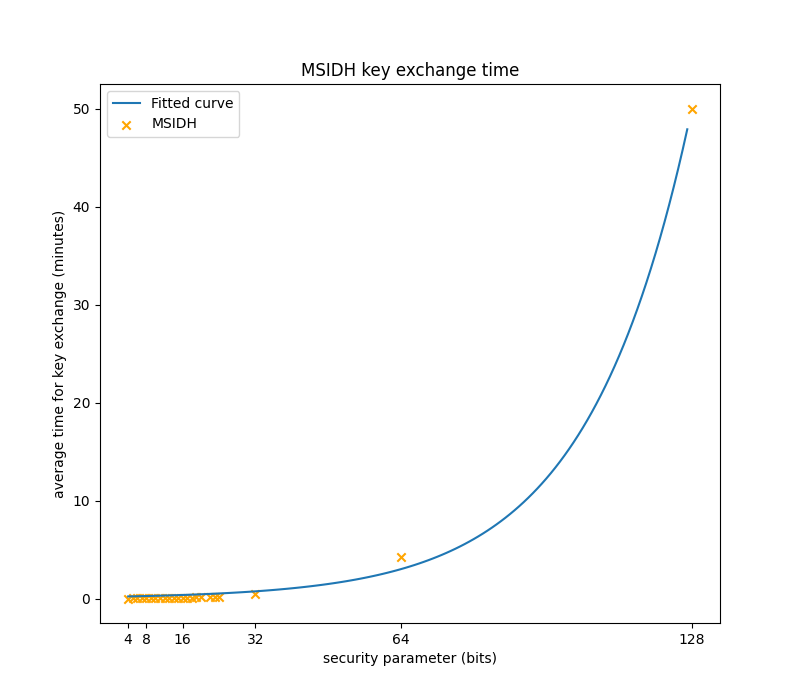
\includegraphics[width=0.7\textwidth]{img/Figure_1.png}
        \caption{Plot of key exchange times}
        \label{fig:ex1}
    \end{figure}

    \begin{figure}
        \centering
        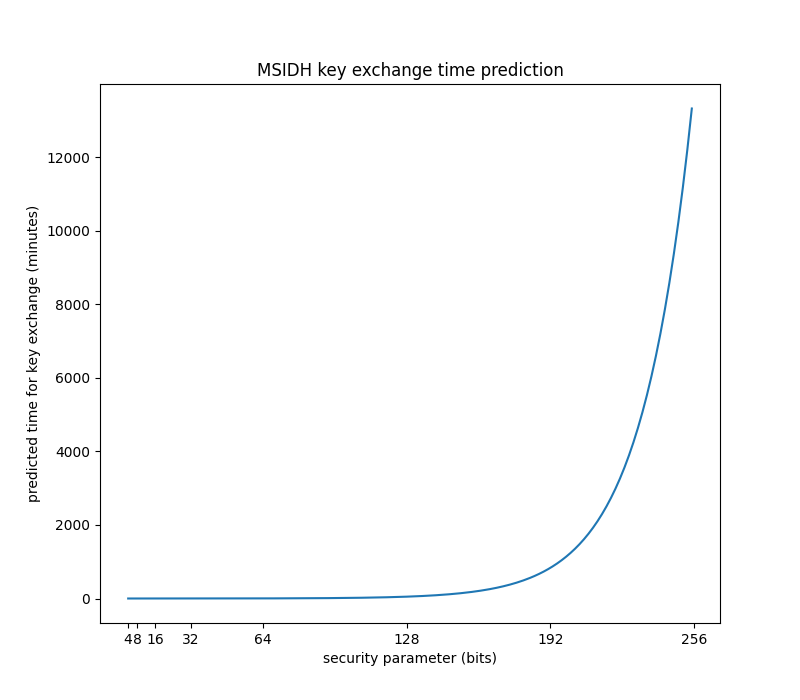
\includegraphics[width=0.7\textwidth]{img/Figure_2.png}
        \caption{Prediction of key exchange times}
        \label{fig:ex2}
    \end{figure}

    To put these results into perspective, we provide runtimes for some NIST security levels of both SIDH \cite{original-sidh} and CSIDH \cite{csidh} (see \autoref{alt_csidh}) in  \autoref{result:more_table}. The SIDH results were generated using the developed implementation of SIDH, while CSIDH was evaluated using the SIBC library \cite{sibc}.


    \begin{table}[!h]
        \label{result:more_table}
        \begin{center}
        \begin{tabular}{| c | c |}
        \hline
        \textbf{Scheme \& Classical security level} & \textbf{Key exchange time (s)} \\ 
        \hline

        SIDH, NIST 1 & 2.852 \\ \hline
        SIDH, NIST 2 & 4.043 \\ \hline
        SIDH, NIST 3 & 6.563 \\ \hline
        SIDH, NIST 5 & 11.26 \\ \hline
        CSIDH, NIST 1 & 17.63 \\ \hline
        CSIDH, NIST 5 & 30.02 \\ \hline
        \hline
        \end{tabular}
        \end{center}
        \caption{Evaluation of some other schemes, on the same machine (10 repetitions)}
    \end{table}

\section{Discussion on the limitations of the SageMath framework}
\label{discussion:limitations}

    In this section, we discuss the difficulties faced during the implementation of this project using SageMath. Comparing the results with the ones achieved in \cite{compression} (reproduced on the same machine as the one used to evaluate this implementation) shows that a more efficient, low-level implementation of the computation of isogenies as described in \cite{algorithms} may yield faster speeds for the key exchange phase. This is one of the downsides of Sage being sometimes too high level for a given goal.

    The SageMath source code (9.8) used to calculate isogenies also seems to have some efficiency issues. One bug in the source code that was found was that the order of the kernel point was calculated at every step of the factored isogeny calculation. A modified version of the source code was implemented\footnote{A copy of the modified source code is included in \href{https://github.com/mrztti/lasec-MSIDH/blob/main/hom\_composite.py}{\texttt{hom\_composite.py}}}. Because the order of the isogenies was already known ($A,B$), function arguments were also included to directly pass the order of the kernel point and skip an (expensive) order calculation.
    
    Furthermore, the decomposed isogenies do not leverage computation using \texttt{velusqrt}. An attempt to modify this was made, but there seems to be a performance issue with the Sage implementation of the algorithm. Indeed, the "naive" Vélu algorithm seems to have much better performance\footnote{This is contrary to what is indicated in the reference guide \textbf{\href{https://doc.sagemath.org/html/en/reference/arithmetic_curves/sage/schemes/elliptic\_curves/hom_velusqrt.html}{here}}}, even for $l > 1000$. 
    In conclusion, the final modifications made to the source code was to remove the order calculation as well as disabling all proofs in SageMath (which was causing a major hangup by checking primality of $p$ multiple times along the calculations).
    
    One other example of a problem encountered came as an attempt to implement multi-core parallel computation for the key generation: currently Sage may seem to be facing some incompatibility with multi-threading\footnote{Running parameter generation on multiple threads yielded a stack trace similar to the one mentioned 
    \textbf{\href{https://github.com/sagemath/cypari2/issues/107}{here}}, seemingly due to some compatibility issues with the \texttt{cypari2} framework
    }. This also has consequences for key exchange, since it could be possible to leverage multiple cores to divide the workload for factored isogenies.
    
    Overall, it would seem like the biggest hope for M-SIDH (and MD-SIDH with even larger isogeny degree) to reach faster practical use speeds would be the development of a low-level, efficient and tailor made implementation of an isogeny computation of degrees in the specific form of these protocols.

%%%%%%%%%%%%%%%%%%%%%%
\chapter{Related Work}
%%%%%%%%%%%%%%%%%%%%%%

Closely related work includes \cite{compression} (Lin, Lin, Cai, Wang, Zhao). It provides an implementation of M-SIDH which includes key compression to reduce the size of the keys. After examining the source code, it seems that the code is not modular, and includes hard coded values at many points of the implementation. An attempt was made at modularizing the code to leverage the low level elliptic curve arithmetic functions implemented in this project, however the lack of documentation and abstraction made the task much too complex. After thoughtful implementation and optimization of the SageMath source code, this project reached similar run times to \cite{compression}, while being generalized to any correct parameter set. 

\label{alt_csidh}
It is also interesting to compare the efficiency of other alternative isogeny based post-quantum cryptosystems: CSIDH \cite{csidh} is one such system. Running an implementation of this scheme \cite{sibc} on the same machine as used to evaluate the implementation of M-SIDH, we find that key exchange for NIST level 1 takes around 15 seconds. Some recent paper even propose and evaluate the use of CSIDH in TLS communication \cite{csidh-tls}, an application far from conceivable with the current performance of M-SIDH.




%%%%%%%%%%%%%%%%%%%%
\chapter{Conclusion}
%%%%%%%%%%%%%%%%%%%%

In this project, we have shown that it is possible to implement M-SIDH as a countermeasure to attacks on SIDH. We provided a standalone, generalized implementation which can be used according to any security parameter $\lambda$. M-SIDH involves working over a finite field of much larger size, with isogenies of much larger degrees, compared to SIDH. Understandably, this implies more computation time for the same level of security, even after optimizing the implementation as much as possible. Even with state of the art algorithms, the key exchange takes almost an hour for NIST security level on a modern machine. Compared to other proposed isogeny based post-quantum cryptosystems like CSIDH. Even if there could be some hope in the development of more efficient isogeny computation, or in building a decentralized trusted system that pre-computes scheme parameters in advance, it is hard to say whether M-SIDH (and as such MD-SIDH) could ever become performance competitive with post-quantum cryptosystems.



\cleardoublepage
\phantomsection
\addcontentsline{toc}{chapter}{Bibliography}
\printbibliography

% Appendices are optional
% \appendix
% %%%%%%%%%%%%%%%%%%%%%%%%%%%%%%%%%%%%%%
% \chapter{How to make a transmogrifier}
% %%%%%%%%%%%%%%%%%%%%%%%%%%%%%%%%%%%%%%
%
% In case you ever need an (optional) appendix.
%
% You need the following items:
% \begin{itemize}
% \item A box
% \item Crayons
% \item A self-aware 5-year old
% \end{itemize}

\end{document}